\documentclass[]{book}
\usepackage{lmodern}
\usepackage{amssymb,amsmath}
\usepackage{ifxetex,ifluatex}
\usepackage{fixltx2e} % provides \textsubscript
\ifnum 0\ifxetex 1\fi\ifluatex 1\fi=0 % if pdftex
  \usepackage[T1]{fontenc}
  \usepackage[utf8]{inputenc}
\else % if luatex or xelatex
  \ifxetex
    \usepackage{mathspec}
  \else
    \usepackage{fontspec}
  \fi
  \defaultfontfeatures{Ligatures=TeX,Scale=MatchLowercase}
\fi
% use upquote if available, for straight quotes in verbatim environments
\IfFileExists{upquote.sty}{\usepackage{upquote}}{}
% use microtype if available
\IfFileExists{microtype.sty}{%
\usepackage{microtype}
\UseMicrotypeSet[protrusion]{basicmath} % disable protrusion for tt fonts
}{}
\usepackage[margin=1in]{geometry}
\usepackage{hyperref}
\hypersetup{unicode=true,
            pdftitle={Modeling Melodic Dictation},
            pdfauthor={David John Baker},
            pdfborder={0 0 0},
            breaklinks=true}
\urlstyle{same}  % don't use monospace font for urls
\usepackage{natbib}
\bibliographystyle{apalike}
\usepackage{color}
\usepackage{fancyvrb}
\newcommand{\VerbBar}{|}
\newcommand{\VERB}{\Verb[commandchars=\\\{\}]}
\DefineVerbatimEnvironment{Highlighting}{Verbatim}{commandchars=\\\{\}}
% Add ',fontsize=\small' for more characters per line
\usepackage{framed}
\definecolor{shadecolor}{RGB}{248,248,248}
\newenvironment{Shaded}{\begin{snugshade}}{\end{snugshade}}
\newcommand{\AlertTok}[1]{\textcolor[rgb]{0.94,0.16,0.16}{#1}}
\newcommand{\AnnotationTok}[1]{\textcolor[rgb]{0.56,0.35,0.01}{\textbf{\textit{#1}}}}
\newcommand{\AttributeTok}[1]{\textcolor[rgb]{0.77,0.63,0.00}{#1}}
\newcommand{\BaseNTok}[1]{\textcolor[rgb]{0.00,0.00,0.81}{#1}}
\newcommand{\BuiltInTok}[1]{#1}
\newcommand{\CharTok}[1]{\textcolor[rgb]{0.31,0.60,0.02}{#1}}
\newcommand{\CommentTok}[1]{\textcolor[rgb]{0.56,0.35,0.01}{\textit{#1}}}
\newcommand{\CommentVarTok}[1]{\textcolor[rgb]{0.56,0.35,0.01}{\textbf{\textit{#1}}}}
\newcommand{\ConstantTok}[1]{\textcolor[rgb]{0.00,0.00,0.00}{#1}}
\newcommand{\ControlFlowTok}[1]{\textcolor[rgb]{0.13,0.29,0.53}{\textbf{#1}}}
\newcommand{\DataTypeTok}[1]{\textcolor[rgb]{0.13,0.29,0.53}{#1}}
\newcommand{\DecValTok}[1]{\textcolor[rgb]{0.00,0.00,0.81}{#1}}
\newcommand{\DocumentationTok}[1]{\textcolor[rgb]{0.56,0.35,0.01}{\textbf{\textit{#1}}}}
\newcommand{\ErrorTok}[1]{\textcolor[rgb]{0.64,0.00,0.00}{\textbf{#1}}}
\newcommand{\ExtensionTok}[1]{#1}
\newcommand{\FloatTok}[1]{\textcolor[rgb]{0.00,0.00,0.81}{#1}}
\newcommand{\FunctionTok}[1]{\textcolor[rgb]{0.00,0.00,0.00}{#1}}
\newcommand{\ImportTok}[1]{#1}
\newcommand{\InformationTok}[1]{\textcolor[rgb]{0.56,0.35,0.01}{\textbf{\textit{#1}}}}
\newcommand{\KeywordTok}[1]{\textcolor[rgb]{0.13,0.29,0.53}{\textbf{#1}}}
\newcommand{\NormalTok}[1]{#1}
\newcommand{\OperatorTok}[1]{\textcolor[rgb]{0.81,0.36,0.00}{\textbf{#1}}}
\newcommand{\OtherTok}[1]{\textcolor[rgb]{0.56,0.35,0.01}{#1}}
\newcommand{\PreprocessorTok}[1]{\textcolor[rgb]{0.56,0.35,0.01}{\textit{#1}}}
\newcommand{\RegionMarkerTok}[1]{#1}
\newcommand{\SpecialCharTok}[1]{\textcolor[rgb]{0.00,0.00,0.00}{#1}}
\newcommand{\SpecialStringTok}[1]{\textcolor[rgb]{0.31,0.60,0.02}{#1}}
\newcommand{\StringTok}[1]{\textcolor[rgb]{0.31,0.60,0.02}{#1}}
\newcommand{\VariableTok}[1]{\textcolor[rgb]{0.00,0.00,0.00}{#1}}
\newcommand{\VerbatimStringTok}[1]{\textcolor[rgb]{0.31,0.60,0.02}{#1}}
\newcommand{\WarningTok}[1]{\textcolor[rgb]{0.56,0.35,0.01}{\textbf{\textit{#1}}}}
\usepackage{longtable,booktabs}
\usepackage{graphicx,grffile}
\makeatletter
\def\maxwidth{\ifdim\Gin@nat@width>\linewidth\linewidth\else\Gin@nat@width\fi}
\def\maxheight{\ifdim\Gin@nat@height>\textheight\textheight\else\Gin@nat@height\fi}
\makeatother
% Scale images if necessary, so that they will not overflow the page
% margins by default, and it is still possible to overwrite the defaults
% using explicit options in \includegraphics[width, height, ...]{}
\setkeys{Gin}{width=\maxwidth,height=\maxheight,keepaspectratio}
\IfFileExists{parskip.sty}{%
\usepackage{parskip}
}{% else
\setlength{\parindent}{0pt}
\setlength{\parskip}{6pt plus 2pt minus 1pt}
}
\setlength{\emergencystretch}{3em}  % prevent overfull lines
\providecommand{\tightlist}{%
  \setlength{\itemsep}{0pt}\setlength{\parskip}{0pt}}
\setcounter{secnumdepth}{5}
% Redefines (sub)paragraphs to behave more like sections
\ifx\paragraph\undefined\else
\let\oldparagraph\paragraph
\renewcommand{\paragraph}[1]{\oldparagraph{#1}\mbox{}}
\fi
\ifx\subparagraph\undefined\else
\let\oldsubparagraph\subparagraph
\renewcommand{\subparagraph}[1]{\oldsubparagraph{#1}\mbox{}}
\fi

%%% Use protect on footnotes to avoid problems with footnotes in titles
\let\rmarkdownfootnote\footnote%
\def\footnote{\protect\rmarkdownfootnote}

%%% Change title format to be more compact
\usepackage{titling}

% Create subtitle command for use in maketitle
\newcommand{\subtitle}[1]{
  \posttitle{
    \begin{center}\large#1\end{center}
    }
}

\setlength{\droptitle}{-2em}
  \title{Modeling Melodic Dictation}
  \pretitle{\vspace{\droptitle}\centering\huge}
  \posttitle{\par}
  \author{David John Baker}
  \preauthor{\centering\large\emph}
  \postauthor{\par}
  \predate{\centering\large\emph}
  \postdate{\par}
  \date{2018-08-29}

\usepackage{booktabs}
\usepackage{amsthm}
\makeatletter
\def\thm@space@setup{%
  \thm@preskip=8pt plus 2pt minus 4pt
  \thm@postskip=\thm@preskip
}
\makeatother

\usepackage{amsthm}
\newtheorem{theorem}{Theorem}[chapter]
\newtheorem{lemma}{Lemma}[chapter]
\theoremstyle{definition}
\newtheorem{definition}{Definition}[chapter]
\newtheorem{corollary}{Corollary}[chapter]
\newtheorem{proposition}{Proposition}[chapter]
\theoremstyle{definition}
\newtheorem{example}{Example}[chapter]
\theoremstyle{definition}
\newtheorem{exercise}{Exercise}[chapter]
\theoremstyle{remark}
\newtheorem*{remark}{Remark}
\newtheorem*{solution}{Solution}
\begin{document}
\maketitle

{
\setcounter{tocdepth}{1}
\tableofcontents
}
\hypertarget{significance-of-the-study}{%
\chapter{Significance of the Study}\label{significance-of-the-study}}

All students pursing a Bachelor's degree in Music from universities
accredited by the National Association of Schools of Music must learn to
take melodic dictation \citep[ Section
VIII.6.B.2.A]{NationalAssociationSchools2018}. Melodic dictation is a
cognitively demanding process that requires students to listen to a
melody, retain it in memory, and then use their knowledge of Western
musical notation in order to recreate the mental image of the melody on
paper in a limited time frame. As of 2018 there are 647 Schools of Music
belonging to National Association of Schools of Music (NASM) CITE
WEBSITE, meaning that hundereds of students every year will be expected
to learn this challenging task as part of their Aural Skills education.
The logic being that as one improves in their abiliy to take melodic
dictation, this practice of critical and active listening develops as a
means to improve one's ability to ``think in music'' and thus become a
more compotent musician. While learning Aural Skills has been a hallmark
of being educated within the Western conservatory tradition, the
rationale behind both the how and why of aural skills is often thought
of as being esoteric. Throughout the past century, people have disagreed
on exactly how one does go about learning a melody with different areas
of research each attacking the problem from a different angle.

Despite its ubiqiquity in curricula within School of Music settings,
research on topics pertain to how aural skills are acquired is limited
at best. {[}Citations here about the cosntant calls butler, klondoski,
pembrook{]} The fields of music theory and cognitive psychology are best
positioned to make progress on this question, but often the skills
required to be well versed ein ither of these subjects are disparate,
published in other journals, and the research with overlap is scarce.
This problem is not new and there have been repeated attempts to bridge
the gap between practioners of aural skills and people in cognitive
psycholgy CITES. Literature from music theory has establisehd conceptual
frameworks regarding aural skills
\citet{karpinskiAuralSkillsAcquisition2000} and the relavint cognitive
psychology literature has explored factors that might contribute to
melodic perception (SCHMUKLER SYNERR 2016 2016), and there exists
applied literature from the world of music education (CITES).

However, despite these siloed areas of research, we as music researchers
do not have an a concrete understanding of exaclty what contributes to
HOW individuals learn melodies (HALPERNBARLETT2010). This is peculiar
since ``how does one learn a melody'' seems to be one of the fundamental
questions to the fields of music theory, music psychology, as well as
music education. Given this lack of understanding, it becomes even more
peculiar that this lack of convergence of evidence is then unable to
provide a solid baseline as to what student in their aural skills
classrooms can be expected to do. (Also something about we should really
know this if we are going to grade people on this ability). While no
single dissertation can solve any problem completely, this dissertation
aims to fill the gap in the literature between aural skills
practitioners (theorists and educators) and music psychologists in order
to reach conclusion that can be applied systematically in pedagogical
contexts. In order to do this I draw both literatures (music and
science) in order to demonstrate how tools from both cognitive
psychology as well as computational musicology can help move both fields
forward. Some line here about if we really want to understand what is
happening we need to know about causal factors going on here and have
experimental manipulation and things like making models of the whole
thing or talk about what Judea Pearl thinks about the ability to do some
sort of causal modeling with diagrams. Great to rely on some sort of
anecdoatal evidence, but if we are going to put things on the line with
our education then we need to be able to make some sort of falsifiable
claims about what we are doing. Can only do that through the lens of
science.

\hypertarget{chapter-overview}{%
\section{Chapter Overview}\label{chapter-overview}}

In this first chapter, I introduce the process of melodic dictation and
discuss factors that would presumably could play a role in taking
melodic dictation. The chapter introduces both a theoretical backgorund
and rationale for using method form both computational musicology and
congitive psychology in order ot answr quesitona bout how individuals
learn melodies. I argue that tools for understanding this best because
as we currently understand it, I see us operating in a Kuhnian normal
science where much can be learned by just using the tools in front of
us. This chapter will clearly outline the factors hypothesized to
contribute to an individual's abilit to learn melodies, incorporating
both individual and musical parameters. The chapter ends with a
discussion some of the philosophical/theoretical problems with
attempting to measure thigns like this (is it just a party trick?) and
establishes that I will be taking a more polymorphic view of
musicianship in order to answer this question.

The second chapter of my dissertation focuses on the history and current
state of aural skills pedagogy.

Tracing back its origins to the practical need to teach musical skills
back with Guido d'Arezzo, I compare and contrast the different
methodological approaches that have been used, along with their goals.

The third chapter discusses previous work that examines individual
factors thought to contribute to one's ability to perform an aural
skills task, and it will discuss results from an experiment contributing
to a discussion of how individual differences could contribute to how a
person learns melodies.

Turning away from individual differences and focusing on musical
features, in the fourth chapter I plan to discuss how music researchers
can use tools from computational musicology as predictive features of
melodies. Inspired by work from computational linguistics and
information theory, recent work in computational musicology has
developed software capable of abstracting features thought to be
important to learning melodies, such as note density and `tonalness'
(Müllensiefen, 2009). Talk a bit about how this has been also looked at
before in the music education community.

While these features have been used in large scale, exploratory studies,
work in this chapter will discuss how these features could be used in
controlled, experimental studies as a stand-in for the intuition many
music pedagogues have when determining difficulty of a melody in a
classroom setting.

In my fifth chapter, I introduce a novel corpus of over 600 digitized
melodies encoded in a queryable format. This dataset will also serve as
a valuable resource for future researchers in music, psychology, and the
digital humanities. This chapter begins with a discussion of the history
of corpus studies, noting their origin outside of music, their current
state in music, and their limitations. This chapter, encapsulating the
encoding process, the sampling criteria, and the situation of corpus
methodologies within the broader research area, will go over summary
data and also talk about how it could be used to generate hypotheses for
future experiemnts (n-gram stuff based on patterns) .

Lastly, in the final chapter, I will synthesize the previous research in
a series of melodic dictation experiments. Stimuli for the experiments
are selected based on the abstracted features of the melodies and are
manipulated as independent variables based on the previous theoretical
literature. I then model responses from the experiments using both
individual factors and musical features in order to predict how well an
individual performs in behavioral tasks similar to some of my previously
published research (Baker \& Müllensiefen, 2017). Here I also note
important caveats in scoring melodic dictation, referencing some other
of my own work on using metrics, such as edit distance (Baker \&
Shanahan, 2018), to discuss similarities between the correct answer and
an individual's attempts at dictation. Results from the final chapter
will be discussed with reference to how findings are applicable to
pedagoges in aural skills settings. Recommendations will be made
building on current conceptual frameworks (Karpinski, 2000).

\hypertarget{intro}{%
\chapter{Theoretical Background and Rationale}\label{intro}}

\hypertarget{what-is-melodic-dictation}{%
\section{What is melodic dictation?}\label{what-is-melodic-dictation}}

\hypertarget{describe-process}{%
\subsection{Describe process}\label{describe-process}}

\hypertarget{karpinski-schematic-of-it-as-verbal-model-problems}{%
\subsection{Karpinski schematic of it (as verbal model,
problems)}\label{karpinski-schematic-of-it-as-verbal-model-problems}}

\hypertarget{verbal-model-has-problems-ok-for-pedagogy}{%
\subsubsection{Verbal model, has problems, OK for
pedagogy}\label{verbal-model-has-problems-ok-for-pedagogy}}

\hypertarget{verbal-model-no-individual-differnces-tho-literture-to-suggest}{%
\subsubsection{Verbal model, no individual differnces tho literture to
suggest}\label{verbal-model-no-individual-differnces-tho-literture-to-suggest}}

\hypertarget{computational-model-to-be-introduced}{%
\subsubsection{Computational model to be
introduced}\label{computational-model-to-be-introduced}}

\hypertarget{clearly-this-is-psychological-problem-with-different-item-level-difficulty}{%
\subsection{Clearly this is psychological problem with different item
level
difficulty}\label{clearly-this-is-psychological-problem-with-different-item-level-difficulty}}

\hypertarget{individual-factors-to-contribute}{%
\subsubsection{Individual Factors to
contribute}\label{individual-factors-to-contribute}}

\hypertarget{musical-factors-to-contribute}{%
\subsubsection{Musical factors to
contribute}\label{musical-factors-to-contribute}}

\hypertarget{make-a-model-of-them}{%
\subsubsection{Make a Model of them}\label{make-a-model-of-them}}

\hypertarget{cognitive-factors-mt-and-it-selection-bias}{%
\section{Cognitive Factors (MT and it selection
bias)}\label{cognitive-factors-mt-and-it-selection-bias}}

\hypertarget{working-memory-capacity}{%
\subsection{Working Memory Capacity}\label{working-memory-capacity}}

\hypertarget{papers-that-suggest-wmc-plays-a-role}{%
\subsubsection{Papers that suggest WMC plays a
role}\label{papers-that-suggest-wmc-plays-a-role}}

\hypertarget{general-fluid-intelligence}{%
\subsection{General Fluid
Intelligence}\label{general-fluid-intelligence}}

\hypertarget{papers-that-suggest-gf-plays-a-role}{%
\subsubsection{Papers that suggest GF plays a
role}\label{papers-that-suggest-gf-plays-a-role}}

\hypertarget{long-term-memory-and-corpus-with-implicit}{%
\subsection{Long term memory and corpus with
implicit}\label{long-term-memory-and-corpus-with-implicit}}

\hypertarget{musical-training}{%
\subsection{Musical Training}\label{musical-training}}

\hypertarget{aural-training}{%
\subsection{Aural Training}\label{aural-training}}

\hypertarget{musical-factors}{%
\section{Musical Factors}\label{musical-factors}}

\hypertarget{not-first-to-model-structure}{%
\subsection{Not first to model
structure}\label{not-first-to-model-structure}}

\hypertarget{early-papers-of-ortmann}{%
\subsection{Early papers of Ortmann}\label{early-papers-of-ortmann}}

\hypertarget{papers-from-1980s}{%
\subsection{Papers from 1980s}\label{papers-from-1980s}}

\hypertarget{buonviri-papers}{%
\subsection{Buonviri Papers}\label{buonviri-papers}}

\hypertarget{fantastic-papers-and-findings}{%
\subsection{FANTASTIC papers and
findings}\label{fantastic-papers-and-findings}}

\hypertarget{modeling-and-polymorphism-of-ability-end-chapter}{%
\section{Modeling and Polymorphism of Ability (End
Chapter)}\label{modeling-and-polymorphism-of-ability-end-chapter}}

\hypertarget{draw-from-mmd-icmcp-on-problems-with-lv-model}{%
\subsection{Draw from MMD ICMCP on problems with LV
model}\label{draw-from-mmd-icmcp-on-problems-with-lv-model}}

\hypertarget{thought-experiments-on-why-musicianship-is-bad-concept-in-general}{%
\subsection{Thought experiments on why musicianship is bad concept in
general}\label{thought-experiments-on-why-musicianship-is-bad-concept-in-general}}

\hypertarget{polymophic-component-process-makes-you-think-about-things-in-models}{%
\subsection{Polymophic, component process makes you think about things
in
models}\label{polymophic-component-process-makes-you-think-about-things-in-models}}

\hypertarget{conclusions}{%
\section{Conclusions}\label{conclusions}}

\hypertarget{clearly-we-have-factors-that-are-thought-to-contribute-need-to-investigate-them-in-full-with-each-chapter}{%
\subsection{Clearly we have factors that are thought to contribute, need
to investigate them in full with each
chapter}\label{clearly-we-have-factors-that-are-thought-to-contribute-need-to-investigate-them-in-full-with-each-chapter}}

\hypertarget{not-before-first-looking-at-why-we-are-doing-it-in-the-first-place-transition-to-chapter-2}{%
\subsection{Not before first looking at why we are doing it in the first
place (--transition to Chapter
2)}\label{not-before-first-looking-at-why-we-are-doing-it-in-the-first-place-transition-to-chapter-2}}

\hypertarget{history-of-aural-skills}{%
\chapter{History of Aural Skills}\label{history-of-aural-skills}}

\hypertarget{thesis-show-that-aural-skills-always-has-practical-end-efficacy-of-representation-of-musical-pitch}{%
\section{Thesis: Show that aural skills always has practical end,
efficacy of representation of musical
pitch}\label{thesis-show-that-aural-skills-always-has-practical-end-efficacy-of-representation-of-musical-pitch}}

\hypertarget{for-i-in-star-aural-people-do}{%
\subsection{for i in star aural people
do}\label{for-i-in-star-aural-people-do}}

\hypertarget{who}{%
\subsection{Who}\label{who}}

\hypertarget{where}{%
\subsection{Where}\label{where}}

\hypertarget{when}{%
\subsection{When}\label{when}}

\hypertarget{what}{%
\subsection{What}\label{what}}

\hypertarget{how-approach-and-goals}{%
\subsection{How (approach and goals)}\label{how-approach-and-goals}}

\hypertarget{why}{%
\subsection{Why}\label{why}}

\hypertarget{guido-darezzo}{%
\subsection{Guido d'Arezzo}\label{guido-darezzo}}

\hypertarget{walerant-via-calvisius}{%
\subsection{Walerant (via Calvisius)}\label{walerant-via-calvisius}}

\hypertarget{banchieri}{%
\subsection{Banchieri}\label{banchieri}}

\hypertarget{cerratto}{%
\subsection{Cerratto}\label{cerratto}}

\hypertarget{penna}{%
\subsection{Penna}\label{penna}}

\hypertarget{zarlino}{%
\subsection{Zarlino}\label{zarlino}}

\hypertarget{quotes-from-schumann}{%
\section{Quotes from Schumann}\label{quotes-from-schumann}}

\hypertarget{carl-seashore-thinking-in-music}{%
\section{Carl Seashore thinking in
music}\label{carl-seashore-thinking-in-music}}

\hypertarget{points-from-karpinski-on-pedagogy}{%
\section{Points from Karpinski on
pedagogy}\label{points-from-karpinski-on-pedagogy}}

\hypertarget{points-from-royal-paper-on-pedagogy}{%
\section{Points from Royal Paper on
pedagogy}\label{points-from-royal-paper-on-pedagogy}}

\hypertarget{solmization-system}{%
\section{Solmization System}\label{solmization-system}}

\hypertarget{really-this-is-all-question-of-efficacy-of-mental-representation-of-musical-pitch}{%
\section{Really this is all question of efficacy of mental
representation of musical
pitch}\label{really-this-is-all-question-of-efficacy-of-mental-representation-of-musical-pitch}}

\hypertarget{individual-differences}{%
\chapter{Individual Differences}\label{individual-differences}}

\hypertarget{why-care-about-cognitive-abilities}{%
\section{Why care about cognitive
abilities}\label{why-care-about-cognitive-abilities}}

\hypertarget{general-intelligence-and-wmc}{%
\subsection{General intelligence and
WMC}\label{general-intelligence-and-wmc}}

\hypertarget{defining-of-terms}{%
\subsection{Defining of terms}\label{defining-of-terms}}

\hypertarget{have-established-that-cognitive-abilities-contribute-to-musical-task-for-journal-article-langauge-repeat}{%
\section{Have established that cognitive abilities contribute to musical
task (for journal article langauge
repeat)}\label{have-established-that-cognitive-abilities-contribute-to-musical-task-for-journal-article-langauge-repeat}}

\hypertarget{general-fluid-intelligence-wmc-training-as-uni-of-polymorphic}{%
\subsection{General Fluid Intelligence, WMC, Training as uni of
polymorphic}\label{general-fluid-intelligence-wmc-training-as-uni-of-polymorphic}}

\hypertarget{remind-the-nature-of-a-musical-dictation-type-task-hear-loop-executive-decision}{%
\section{Remind the nature of a musical dictation type task (hear, loop,
executive
decision)}\label{remind-the-nature-of-a-musical-dictation-type-task-hear-loop-executive-decision}}

\hypertarget{this-is-wmc-task-gf-has-problems-although-high-level-link-with-gf-problematic-wmc-models-at-level-of-process-of-md}{%
\subsection{This is WMC task, gf has problems (Although high level link
with gf, problematic, WMC models at level of process of
md)}\label{this-is-wmc-task-gf-has-problems-although-high-level-link-with-gf-problematic-wmc-models-at-level-of-process-of-md}}

\hypertarget{berz-1994-noticed-it-first}{%
\subsubsection{Berz 1994 noticed it
first}\label{berz-1994-noticed-it-first}}

\hypertarget{williamson-baddely-hitch-suggest-maybe-musical-loop}{%
\subsubsection{Williamson Baddely Hitch suggest maybe musical
loop}\label{williamson-baddely-hitch-suggest-maybe-musical-loop}}

\hypertarget{even-cowan-labs-wonder-how-different-li-cowan-saults}{%
\subsubsection{Even Cowan labs wonder how different (Li Cowan Saults
)}\label{even-cowan-labs-wonder-how-different-li-cowan-saults}}

\hypertarget{wmc-has-been-misused-in-music-education-theory-pedagogy-aural-literature-and-deserves-attention}{%
\section{WMC has been misused in music education, theory, pedagogy,
aural literature and deserves
attention}\label{wmc-has-been-misused-in-music-education-theory-pedagogy-aural-literature-and-deserves-attention}}

\hypertarget{problems-with-chunking}{%
\subsection{Problems with chunking}\label{problems-with-chunking}}

\hypertarget{mistake-with-miller-1956-he-did-not-mean-7-items}{%
\subsubsection{Mistake with Miller 1956, he did not mean 7
items}\label{mistake-with-miller-1956-he-did-not-mean-7-items}}

\hypertarget{broadbent-1956-more-of-why-its-more-like-3-4}{%
\subsubsection{Broadbent 1956 more of why its more like
3-4}\label{broadbent-1956-more-of-why-its-more-like-3-4}}

\hypertarget{problems-with-using-capacity-limit-literature}{%
\subsection{Problems with using capacity limit
literature}\label{problems-with-using-capacity-limit-literature}}

\hypertarget{see-cowan-2005-page-80}{%
\subsubsection{See Cowan 2005 page 80}\label{see-cowan-2005-page-80}}

\hypertarget{musical-order-is-always-serial-effects}{%
\subsubsection{Musical order is always serial
effects}\label{musical-order-is-always-serial-effects}}

\hypertarget{should-be-using-cowan-model-because-of-these-things-zooming-or-discuss-within-baddely-hitchatkinson-shriff}{%
\subsection{Should be using Cowan model because of these things
(zooming) or discuss within Baddely Hitch/Atkinson
Shriff}\label{should-be-using-cowan-model-because-of-these-things-zooming-or-discuss-within-baddely-hitchatkinson-shriff}}

\hypertarget{one-note-does-not-mean-one-unit-in-memory}{%
\subsection{One Note does not mean one unit in
memory!}\label{one-note-does-not-mean-one-unit-in-memory}}

\hypertarget{confounded-by-corpus-distributions}{%
\subsection{Confounded by corpus
distributions}\label{confounded-by-corpus-distributions}}

\hypertarget{lack-of-understanding-all-aural-skills-are-those-that-engage-wmc-lvh-says-many-students-have-wmc-deficits-increase-memory}{%
\subsection{Lack of understanding (all aural skills are those that
engage WMC, LVH says many students have WMC deficits, ``increase
memory'')}\label{lack-of-understanding-all-aural-skills-are-those-that-engage-wmc-lvh-says-many-students-have-wmc-deficits-increase-memory}}

\hypertarget{point-i-am-making-is-that-if-youre-going-to-do-it-do-it-well.}{%
\subsection{Point I am making is that if you're going to do it, do it
well.}\label{point-i-am-making-is-that-if-youre-going-to-do-it-do-it-well.}}

\hypertarget{know-wmc-plays-a-role-sense-pertain-execute-should-be-able-to-pick-up-in-experiment-close-to-md}{%
\section{Know WMC plays a role, sense, pertain, execute, should be able
to pick up in experiment close to
MD}\label{know-wmc-plays-a-role-sense-pertain-execute-should-be-able-to-pick-up-in-experiment-close-to-md}}

\hypertarget{gold-msi-melodic-memory-and-beat-perception-test}{%
\section{Gold-MSI melodic Memory and beat perception
test}\label{gold-msi-melodic-memory-and-beat-perception-test}}

\hypertarget{what-is-gold-msi}{%
\subsection{What is gold MSI}\label{what-is-gold-msi}}

\hypertarget{what-are-issues-i-want-to-talk-about-with-psychometrics}{%
\subsection{What are issues I want to talk about with
psychometrics}\label{what-are-issues-i-want-to-talk-about-with-psychometrics}}

\hypertarget{describe-test-in-detail-and-why-its-what-were-after-here}{%
\subsection{Describe test in detail and WHY it's what we're after
here}\label{describe-test-in-detail-and-why-its-what-were-after-here}}

\hypertarget{not-exactly-mmd-but-most-people-would-say-similar-skill-sets}{%
\subsubsection{not exactly mmd, but most people would say similar skill
sets}\label{not-exactly-mmd-but-most-people-would-say-similar-skill-sets}}

\hypertarget{also-before-getting-dirtyneed-experimental-desing-with-less-response-options-cowan-saults-elliott-moreano-2002}{%
\subsubsection{also before getting dirty,need experimental desing with
less response options (Cowan, Saults, Elliott, Moreano
2002)}\label{also-before-getting-dirtyneed-experimental-desing-with-less-response-options-cowan-saults-elliott-moreano-2002}}

\hypertarget{if-we-accept-these-dvs-then-we-should-be-able-to-predict-them-with-self-reports-and-measures-of-wmc-and-gf}{%
\section{IF we accept these DVs, THEN we should be able to predict them
with self reports and measures of WMC and
gf}\label{if-we-accept-these-dvs-then-we-should-be-able-to-predict-them-with-self-reports-and-measures-of-wmc-and-gf}}

\hypertarget{do-this-with-hierarchical-lvm-ala-elliott-paper}{%
\section{Do this with hierarchical LVM ala Elliott
paper}\label{do-this-with-hierarchical-lvm-ala-elliott-paper}}

\hypertarget{versions-of-this-paper-at-icmpc}{%
\subsection{Versions of this paper at
ICMPC}\label{versions-of-this-paper-at-icmpc}}

\hypertarget{exploratory-in-that-tried-a-few-different-models-high-type-i-error-but-whatever}{%
\subsection{Exploratory in that tried a few different models (high type
I error but
whatever)}\label{exploratory-in-that-tried-a-few-different-models-high-type-i-error-but-whatever}}

\hypertarget{overview-of-experiment-cross-sectional-design}{%
\section{Overview of Experiment (cross sectional
design)}\label{overview-of-experiment-cross-sectional-design}}

\hypertarget{participants}{%
\subsection{Participants}\label{participants}}

\hypertarget{materials}{%
\subsection{Materials}\label{materials}}

\hypertarget{procedure}{%
\subsection{Procedure}\label{procedure}}

\hypertarget{results}{%
\subsection{Results}\label{results}}

\hypertarget{descriptive-correlational}{%
\subsubsection{Descriptive,
Correlational}\label{descriptive-correlational}}

\hypertarget{modeling}{%
\subsubsection{Modeling}\label{modeling}}

\hypertarget{discussion}{%
\subsection{Discussion}\label{discussion}}

\hypertarget{review-of-the-goals}{%
\subsubsection{Review of the Goals}\label{review-of-the-goals}}

\hypertarget{what-were-best-model-fits}{%
\subsubsection{What were best model
fits}\label{what-were-best-model-fits}}

\hypertarget{clear-effect-of-wmc}{%
\subsubsection{Clear effect of WMC}\label{clear-effect-of-wmc}}

\hypertarget{what-if-we-are-just-measuring-wmc}{%
\subsubsection{What if we are just measuring
WMC?}\label{what-if-we-are-just-measuring-wmc}}

\hypertarget{obvs-need-this-for-futre-studies}{%
\subsubsection{Obvs need this for futre
studies}\label{obvs-need-this-for-futre-studies}}

\hypertarget{need-to-use-something-to-go-above-and-beyond-baseline-transition-to-corpus-as-memory-and-n-gram}{%
\subsubsection{Need to use something to go above and beyond baseline
(--transition to corpus as memory and
n-gram)}\label{need-to-use-something-to-go-above-and-beyond-baseline-transition-to-corpus-as-memory-and-n-gram}}

\hypertarget{future-verbal-theoretical-and-computational-models-should-involve-capacity-measures-limits}{%
\subsubsection{Future verbal theoretical and computational models should
involve capacity measures
(limits)}\label{future-verbal-theoretical-and-computational-models-should-involve-capacity-measures-limits}}

\hypertarget{computation-chapter}{%
\chapter{Computation Chapter}\label{computation-chapter}}

\hypertarget{humans-like-patterns-and-are-very-good-at-picking-them-up}{%
\section{Humans like patterns and are very good at picking them
up}\label{humans-like-patterns-and-are-very-good-at-picking-them-up}}

\hypertarget{we-learn-things-implicitly}{%
\subsection{We learn things
implicitly}\label{we-learn-things-implicitly}}

\hypertarget{we-can-represent-that-implicit-knowledge-with-a-corpus}{%
\subsection{We can represent that implicit knowledge with a
corpus}\label{we-can-represent-that-implicit-knowledge-with-a-corpus}}

\hypertarget{pre-musical-corpora}{%
\section{Pre-Musical Corpora}\label{pre-musical-corpora}}

\hypertarget{information-theory}{%
\subsection{Information Theory}\label{information-theory}}

\hypertarget{computational-linguistics-as-front-runner}{%
\subsection{Computational Linguistics as front
runner}\label{computational-linguistics-as-front-runner}}

\hypertarget{musical-corpora}{%
\section{Musical Corpora}\label{musical-corpora}}

\hypertarget{history-of-musical-corpora}{%
\subsection{History of Musical
Corpora}\label{history-of-musical-corpora}}

\hypertarget{fun-old-computational-music-papers}{%
\subsubsection{Fun old computational music
papers}\label{fun-old-computational-music-papers}}

\hypertarget{corpora-that-are-often-used}{%
\subsubsection{Corpora that are often
used}\label{corpora-that-are-often-used}}

\hypertarget{static-vs-dynamic-models-of-feature-abstraction-daniel-slides}{%
\subsubsection{Static vs Dynamic models of feature abstraction (daniel
slides?)}\label{static-vs-dynamic-models-of-feature-abstraction-daniel-slides}}

\hypertarget{fantastic}{%
\subsection{FANTASTIC}\label{fantastic}}

\hypertarget{static}{%
\subsubsection{static}\label{static}}

\hypertarget{ml-approach-gets-it-right}{%
\subsubsection{ML approach gets it
right}\label{ml-approach-gets-it-right}}

\hypertarget{simple-to-understand}{%
\subsubsection{simple to understand}\label{simple-to-understand}}

\hypertarget{can-abstract-features-be-percieved}{%
\subsubsection{Can abstract features be
percieved?}\label{can-abstract-features-be-percieved}}

\hypertarget{note-density}{%
\subparagraph{Note density}\label{note-density}}

\hypertarget{contour-variation}{%
\subparagraph{Contour variation}\label{contour-variation}}

\hypertarget{tonalness}{%
\subparagraph{Tonalness}\label{tonalness}}

\hypertarget{weird-computational-measures}{%
\subparagraph{weird computational
measures}\label{weird-computational-measures}}

\hypertarget{idyom-as-representation-of-musical-materials}{%
\subsection{IDyOM as representation of musical
materials}\label{idyom-as-representation-of-musical-materials}}

\hypertarget{n-gram-models}{%
\subsubsection{n-gram models}\label{n-gram-models}}

\hypertarget{mirrors-human-behavior}{%
\subsubsection{mirrors human behavior}\label{mirrors-human-behavior}}

\hypertarget{melody}{%
\subparagraph{melody}\label{melody}}

\hypertarget{harmony}{%
\subparagraph{harmony}\label{harmony}}

\hypertarget{so-what}{%
\section{So What?}\label{so-what}}

\hypertarget{other-research-chapt-3-suggest-need-to-move-beyond-cognitive-measures}{%
\subsubsection{Other research (Chapt 3) suggest need to move beyond
cognitive
measures}\label{other-research-chapt-3-suggest-need-to-move-beyond-cognitive-measures}}

\hypertarget{can-operationalize-item-level-items-contextually-with-a-corpus}{%
\subsubsection{Can operationalize item level items contextually with a
corpus}\label{can-operationalize-item-level-items-contextually-with-a-corpus}}

\hypertarget{if-features-are-real-they-should-effect-dictation-chater-6}{%
\subsubsection{IF features are real, they should effect dictation
(Chater
6)}\label{if-features-are-real-they-should-effect-dictation-chater-6}}

\hypertarget{not-only-important-for-one-off-but-then-would-be-incorporated-into-computational-learning-models-chapter-6}{%
\subsubsection{Not only important for one off, but then would be
incorporated into computational learning models (Chapter
6)}\label{not-only-important-for-one-off-but-then-would-be-incorporated-into-computational-learning-models-chapter-6}}

\hypertarget{we-need-new-materials}{%
\subsubsection{We need new materials}\label{we-need-new-materials}}

\hypertarget{hello-corpus}{%
\chapter{Hello, Corpus}\label{hello-corpus}}

\hypertarget{brief-review-of-chapter-4-on-corpus-language-to-reflect-journal-submission}{%
\section{Brief review of Chapter 4 on corpus (Language to reflect
journal
submission)}\label{brief-review-of-chapter-4-on-corpus-language-to-reflect-journal-submission}}

\hypertarget{corpus-outside-of-music}{%
\subsection{Corpus outside of music}\label{corpus-outside-of-music}}

\hypertarget{corpus-in-music}{%
\subsection{Corpus in Music}\label{corpus-in-music}}

\hypertarget{the-point-is-that-it-implicitly-represents-humand-knowledge}{%
\subsection{The point is that it implicitly represents humand
knowledge}\label{the-point-is-that-it-implicitly-represents-humand-knowledge}}

\hypertarget{idyom-1}{%
\subsection{IDyOM 1}\label{idyom-1}}

\hypertarget{idyom-2}{%
\subsection{IDyOM 2}\label{idyom-2}}

\hypertarget{idyom-3}{%
\subsection{IDyOM 3}\label{idyom-3}}

\hypertarget{huron-suggestions-that-starts-of-melodies-relate-to-mental-rotaiton}{%
\subsection{Huron suggestions that starts of melodies relate to mental
rotaiton}\label{huron-suggestions-that-starts-of-melodies-relate-to-mental-rotaiton}}

\hypertarget{other-huron-claims}{%
\subsection{Other Huron claims}\label{other-huron-claims}}

\hypertarget{note-problem-with-using-corpus-is-making-corpus}{%
\section{Note problem with using corpus is making
corpus}\label{note-problem-with-using-corpus-is-making-corpus}}

\hypertarget{many-are-used-on-essen}{%
\subsection{Many are used on Essen}\label{many-are-used-on-essen}}

\hypertarget{brinkman-says-essen-sucks}{%
\subsection{Brinkman says Essen Sucks}\label{brinkman-says-essen-sucks}}

\hypertarget{if-going-to-make-generlizable-claims-need-to-always-have-new-data}{%
\subsection{If going to make generlizable claims, need to always have
new
data}\label{if-going-to-make-generlizable-claims-need-to-always-have-new-data}}

\hypertarget{solem-duty-to-encode-and-report-on-corpus}{%
\section{Solem duty to encode and report on
corpus}\label{solem-duty-to-encode-and-report-on-corpus}}

\hypertarget{justin-london-article-on-what-makes-it-into-a-corpsu}{%
\subsection{Justin London Article on what makes it into a
corpsu}\label{justin-london-article-on-what-makes-it-into-a-corpsu}}

\hypertarget{though-i-just-encoded-the-whole-thing-because-in-my-heart-of-hearts-im-a-bayesian}{%
\subsection{Though I just encoded the whole thing because in my heart of
hearts I'm a
Bayesian}\label{though-i-just-encoded-the-whole-thing-because-in-my-heart-of-hearts-im-a-bayesian}}

\hypertarget{the-corpus}{%
\section{The Corpus}\label{the-corpus}}

\hypertarget{history-of-sight-singign-books}{%
\subsection{History of Sight Singign
books}\label{history-of-sight-singign-books}}

\hypertarget{assumed-to-be-where-long-term-store-comes-from-adumbrate-computational-model}{%
\subsection{Assumed to be where long term store comes from (adumbrate
computational
model)}\label{assumed-to-be-where-long-term-store-comes-from-adumbrate-computational-model}}

\hypertarget{lots-of-melodies-in-ascending-order-of-difficulty-grouped-appropriately-though-utah-guy}{%
\subsection{Lots of melodies in ascending order of difficulty, grouped
appropriately though? Utah
guy}\label{lots-of-melodies-in-ascending-order-of-difficulty-grouped-appropriately-though-utah-guy}}

\hypertarget{why-i-encoded-it-in-xml}{%
\subsection{Why I encoded it in XML}\label{why-i-encoded-it-in-xml}}

\hypertarget{is-it-legal}{%
\subsection{Is it legal?}\label{is-it-legal}}

\hypertarget{descriptive-stats-of-corpus}{%
\section{Descriptive Stats of
Corpus}\label{descriptive-stats-of-corpus}}

\hypertarget{why-1}{%
\subsection{Why?}\label{why-1}}

\hypertarget{for-pedagogical-purposes}{%
\subsubsection{For pedagogical
purposes}\label{for-pedagogical-purposes}}

\hypertarget{for-experimental-purposes}{%
\subsubsection{For experimental
purposes}\label{for-experimental-purposes}}

\hypertarget{for-computational-idexing-get-me-melody-with-x-tonal-score}{%
\subsubsection{For computational idexing (get me melody with x tonal
score)}\label{for-computational-idexing-get-me-melody-with-x-tonal-score}}

\hypertarget{could-serve-as-representation-of-implicitly-learned-expectations-for-future-modeling}{%
\subsubsection{Could serve as representation of implicitly learned
expectations for future
modeling}\label{could-serve-as-representation-of-implicitly-learned-expectations-for-future-modeling}}

\hypertarget{feature-level}{%
\subsection{Feature Level}\label{feature-level}}

\hypertarget{what-features-are-normally-distributed}{%
\subsubsection{What features are normally
distributed}\label{what-features-are-normally-distributed}}

\hypertarget{correlated-feature-problem}{%
\subsubsection{Correlated feature
problem}\label{correlated-feature-problem}}

\hypertarget{big-facet-wrap-of-the-whole-thing}{%
\subsubsection{big \textasciitilde{}facet wrap of the whole
thing}\label{big-facet-wrap-of-the-whole-thing}}

\hypertarget{could-do-dimensonality-reduction-baker-harrison-others-but-then-loose-understanding}{%
\subsubsection{Could do dimensonality reduction (Baker, Harrison,
others) but then loose
understanding}\label{could-do-dimensonality-reduction-baker-harrison-others-but-then-loose-understanding}}

\hypertarget{n-gram}{%
\subsection{n-gram}\label{n-gram}}

\hypertarget{big-solfege-n-gram-table}{%
\subsubsection{Big solfege n-gram
table}\label{big-solfege-n-gram-table}}

\hypertarget{dependent-on-representation-notes-solfege-mint}{%
\subsubsection{Dependent on representation (notes, solfege,
mint)}\label{dependent-on-representation-notes-solfege-mint}}

\hypertarget{shiny-app-of-n-gram-heatmap-with-peter}{%
\subsubsection{Shiny app of n-gram heatmap with
Peter}\label{shiny-app-of-n-gram-heatmap-with-peter}}

\hypertarget{idea-would-be-that-hotter-n-grams-lend-them-selves-to-better-chunking-but-need-better-word-than-chunking}{%
\subsubsection{Idea would be that hotter n-grams lend them selves to
better chunking (but need better word than
chunking)}\label{idea-would-be-that-hotter-n-grams-lend-them-selves-to-better-chunking-but-need-better-word-than-chunking}}

\hypertarget{final-words}{%
\chapter{Final Words}\label{final-words}}

We have finished a nice book.

You can label chapter and section titles using \texttt{\{\#label\}}
after them, e.g., we can reference Chapter \ref{intro}. If you do not
manually label them, there will be automatic labels anyway, e.g.,
Chapter \ref{methods}.

Figures and tables with captions will be placed in \texttt{figure} and
\texttt{table} environments, respectively.

\begin{Shaded}
\begin{Highlighting}[]
\KeywordTok{par}\NormalTok{(}\DataTypeTok{mar =} \KeywordTok{c}\NormalTok{(}\DecValTok{4}\NormalTok{, }\DecValTok{4}\NormalTok{, }\FloatTok{.1}\NormalTok{, }\FloatTok{.1}\NormalTok{))}
\KeywordTok{plot}\NormalTok{(pressure, }\DataTypeTok{type =} \StringTok{'b'}\NormalTok{, }\DataTypeTok{pch =} \DecValTok{19}\NormalTok{)}
\end{Highlighting}
\end{Shaded}

\begin{figure}

{\centering 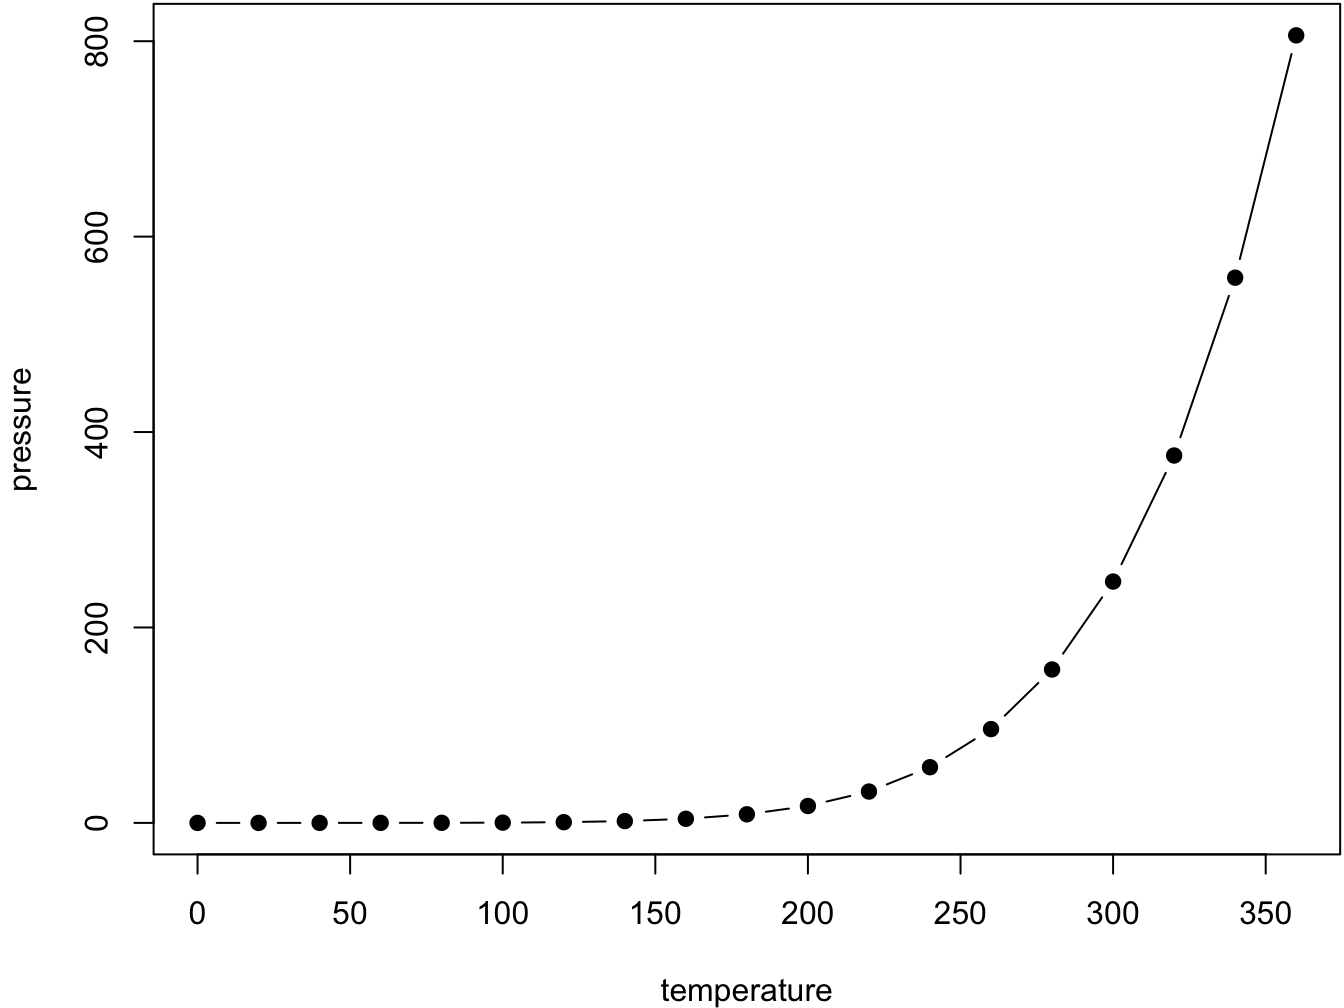
\includegraphics[width=0.8\linewidth]{bookdown-demo_files/figure-latex/nice-fig-1} 

}

\caption{Here is a nice figure!}\label{fig:nice-fig}
\end{figure}

Reference a figure by its code chunk label with the \texttt{fig:}
prefix, e.g., see Figure \ref{fig:nice-fig}. Similarly, you can
reference tables generated from \texttt{knitr::kable()}, e.g., see Table
\ref{tab:nice-tab}.

\begin{Shaded}
\begin{Highlighting}[]
\NormalTok{knitr}\OperatorTok{::}\KeywordTok{kable}\NormalTok{(}
  \KeywordTok{head}\NormalTok{(iris, }\DecValTok{20}\NormalTok{), }\DataTypeTok{caption =} \StringTok{'Here is a nice table!'}\NormalTok{,}
  \DataTypeTok{booktabs =} \OtherTok{TRUE}
\NormalTok{)}
\end{Highlighting}
\end{Shaded}

\begin{table}

\caption{\label{tab:nice-tab}Here is a nice table!}
\centering
\begin{tabular}[t]{rrrrl}
\toprule
Sepal.Length & Sepal.Width & Petal.Length & Petal.Width & Species\\
\midrule
5.1 & 3.5 & 1.4 & 0.2 & setosa\\
4.9 & 3.0 & 1.4 & 0.2 & setosa\\
4.7 & 3.2 & 1.3 & 0.2 & setosa\\
4.6 & 3.1 & 1.5 & 0.2 & setosa\\
5.0 & 3.6 & 1.4 & 0.2 & setosa\\
\addlinespace
5.4 & 3.9 & 1.7 & 0.4 & setosa\\
4.6 & 3.4 & 1.4 & 0.3 & setosa\\
5.0 & 3.4 & 1.5 & 0.2 & setosa\\
4.4 & 2.9 & 1.4 & 0.2 & setosa\\
4.9 & 3.1 & 1.5 & 0.1 & setosa\\
\addlinespace
5.4 & 3.7 & 1.5 & 0.2 & setosa\\
4.8 & 3.4 & 1.6 & 0.2 & setosa\\
4.8 & 3.0 & 1.4 & 0.1 & setosa\\
4.3 & 3.0 & 1.1 & 0.1 & setosa\\
5.8 & 4.0 & 1.2 & 0.2 & setosa\\
\addlinespace
5.7 & 4.4 & 1.5 & 0.4 & setosa\\
5.4 & 3.9 & 1.3 & 0.4 & setosa\\
5.1 & 3.5 & 1.4 & 0.3 & setosa\\
5.7 & 3.8 & 1.7 & 0.3 & setosa\\
5.1 & 3.8 & 1.5 & 0.3 & setosa\\
\bottomrule
\end{tabular}
\end{table}

You can write citations, too. For example, we are using the
\textbf{bookdown} package \citep{R-bookdown} in this sample book, which
was built on top of R Markdown and \textbf{knitr} \citep{xie2015}.

\hypertarget{reference-log}{%
\chapter{Reference Log}\label{reference-log}}

\hypertarget{to-incorporate}{%
\section{To Incorporate}\label{to-incorporate}}

\begin{itemize}
\tightlist
\item
  \citep{margulisModelMelodicExpectation2005} -- Margulis Model
\item
  \citep{nicholsScoreOneJazz2018} -- Specialty jazz background helps in
  tasks, WMC
\item
  \citep{NASM201718HandbookPdf2018} -- Fix intext
\item
  \citep{schumann1860musikalische} -- Quote about why people should do
  ear training
\item
  \citep{smith1934solfege} -- Quote from K2001 about why people should
  do ear training
\item
  \citep{longRelationshipsPitchMemory1977} -- Musical Characteristics
  predict memory
\item
  \citep{taylorStrategiesMemoryShort1983} -- Great citation that lots of
  things change memory, even structural!
\item
  \citep{tallaricoStudyThreePhase1974} -- Long boring talk on STM, LTM
\item
  \citep{ouraConstructingRepresentationMelody1991a} -- Awful
  experimental design that says people use structual tones
\item
  \citep{buonviriExplorationUndergraduateMusic2014} -- Call for
  experimental, suggestions as to what factors might contribute, use of
  deductive reasoning, qualitative
\item
  \citep{buonviriEffectsPreparatorySinging2015} -- People need to focus
  right away, not establish, distractors
\item
  \citep{buonviriEffectsMusicNotation2015} -- Showing people visual
  music does not help much.
\item
  \citep{buonviriEffectsTwoListening2017} -- Listening helps with other
  things, no best strategy in terms of writing
\item
  \citep{buonviriMelodicDictationInstruction2015} -- Literature to say
  people are bad at teaching melodic dictation and we don't know a lot
  about it, also interesting stuff about what solfege systems people use
\item
  \citep{davidbutlerWhyGulfMusic1997a} -- Call for music educators to do
  aural skills research, notes problem with aural skills pedagogy in
  lack of direction, also nice Nicholas Cook quotes on point of theory
\item
  \citep{furbyEffectsPeerTutoring2016} -- music ed study with weird
  stats, has references to follow up on with advantages of pitch systems
  and people who reccomend things for sight singing
\item
  \citep{pembrookInterferenceTranscriptionProcess1986} -- Effects of
  melodies, also how people do it. Interesting that they too effect of
  melodies, but talka bout things in terms of notes and not in terms of
  information content. Thought ot have an experiment where the n-grams
  that are more common are easier to write down. Lots of good charts
  too.
\item
  \citep{paneyEffectDirectingAttention2016} -- It's not good if you tell
  people what to do when they are dictating, article has a lot of good
  review for dictation materials to add to the `toRead' folder.
\item
  \citep{fournierCognitiveStrategiesSightsinging2017a} -- Good
  references that people are awful at Aural Skills, Also suggestions
  that people are not that great at transfer, and some stuff to suggest
  academic abililty is intertwined in all of this. Good reference for
  when starting to talk about untangling the mess that is aural skills.
\item
  \citep[ 1995]{berzWorkingMemoryMusic} -- Add on a new module to the
  WMC model of baddel with music, presents some evidence for why this
  theoretically should be included, but actually takes examples of
  dictation. A lot of this article felt like things that i was
  reinventing\ldots{}not good.
\item
  \citep{atkinsonSomeThoughtsOnTrying} -- Proof some other people are
  starting to think in terms of pedagogical schemas
\item
  \citep{klonoskiPerceptualLearningHierarchy2000} -- Music cognition
  needs to talk to aural skills more, also need to unbind theory routine
  with aural skills and think of things more as in a perceptual learning
  hierarchy
\item
  \citep{klonoskiImprovingDictationAuralSkills2006} -- great quotes that
  when people get something wrong with aural skills, what does that even
  mean, lack of transfer effects, article ends with ways to get better
  at things
\item
  \citep{pembrookSendHelpAural1990} -- Survey of what people in the late
  1980s were doing in terms of aural skills pedagogy
\item
  \citep{karpinskiModelMelodicPerception1990} -- addresses why Gary
  Karpinski thinks we should teach melodic dictation
\item
  \citep{potterIdentifyingSucessfulDictation} -- dictation teacher
  surprised that people don't keep up their dictaiton skills quote
\end{itemize}

\hypertarget{chapter-3}{%
\section{Chapter 3}\label{chapter-3}}

\begin{itemize}
\item
  \citep{cowanWorkingMemoryCapacity2005} -- This book will probably
  serve as cornerstone of chapter in terms of creating relevant
  literature in addition to EE course readings on WMC. Provides history
  of WMC models and notes how attention based model as opposed to
  Baddely loop might actually be better theoretical model for talking
  about fact that WMC could just be something related to attention if
  not that. Provides extensive listing on problems with chunking that
  are all relevant to music, but then also supports it. Shows that
  Miller 1956 is a generally bad citation, own author even says that in
  Miller 1989 (check and add) and says limit is probably about 4 (use
  Cowan 2001 for ctation find that). Lots of good ideas like how music
  is always serial recall, examples of how to model the process, great
  discussions on zooming out and categorical nature of music within span
  of WMC ideas.
\item
  \citep{ockelfordMusicModuleWorking2007} -- uses case of savant to
  argue bits of Berz WM Music Model
\end{itemize}

\bibliography{book.bib,packages.bib}


\end{document}
